%!TEX root = Manuscript.tex

\chapter{Comparison between $SIFT_{ours}$ and $SIFT_{orig}$}
\label{chap:appendix1}

\section{Comparison on method $SIFT_{ImgPairs}$}

\begin{figure*}[htbp]
	\scriptsize 
	\begin{center}
		\subfigure[Image pair]{
			\begin{minipage}[t]{0.48\linewidth}
				\centering
				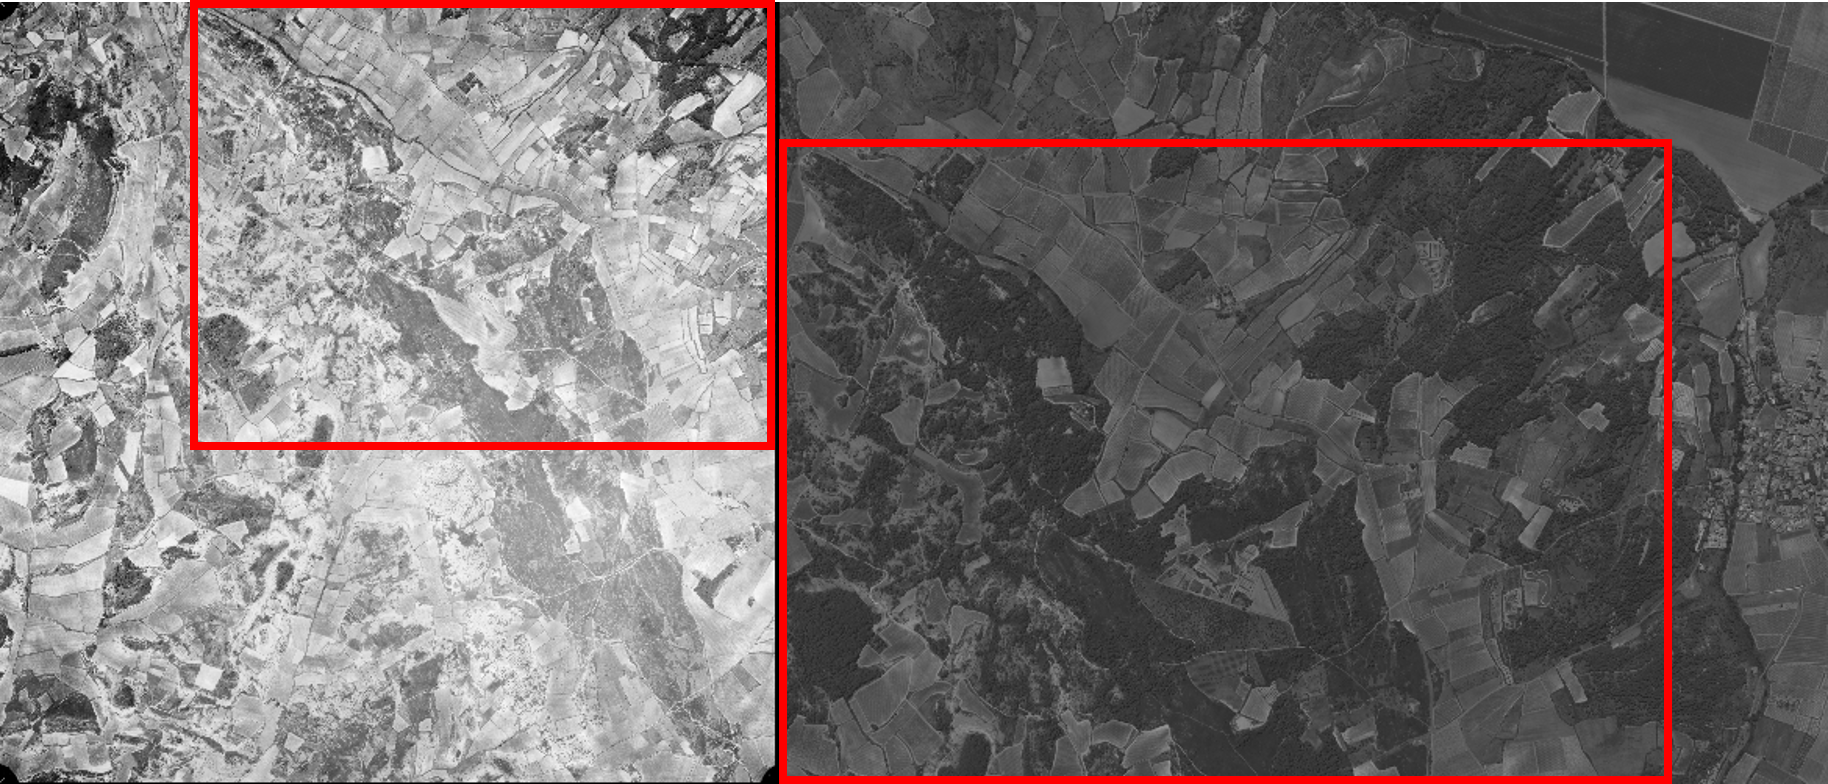
\includegraphics[width=7.5cm]{images/appendix/OIS-Reech_IGNF_PVA_1-0__1971-06-21__C2844-0141_1971_FR2117_1124_15FD3425x00034_02911.png}
			\end{minipage}%
		}
		\subfigure[Match number (\textit{ImgPairs})]{
			\begin{minipage}[t]{0.48\linewidth}
				\centering
				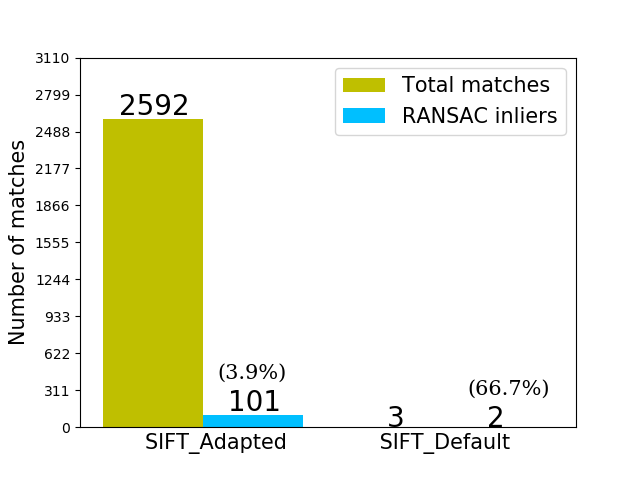
\includegraphics[width=4.8cm]{images/appendix/PlotCurves-SIFTComp_OIS-Reech_IGNF_PVA_1-0__1971-06-21__C2844-0141_1971_FR2117_1124_15FD3425x00034_02911.png}
			\end{minipage}%
		}
		\subfigure[$SIFT_{ours}^{RANSAC Inliers}$]{
			\begin{minipage}[t]{0.48\linewidth}
				\centering
				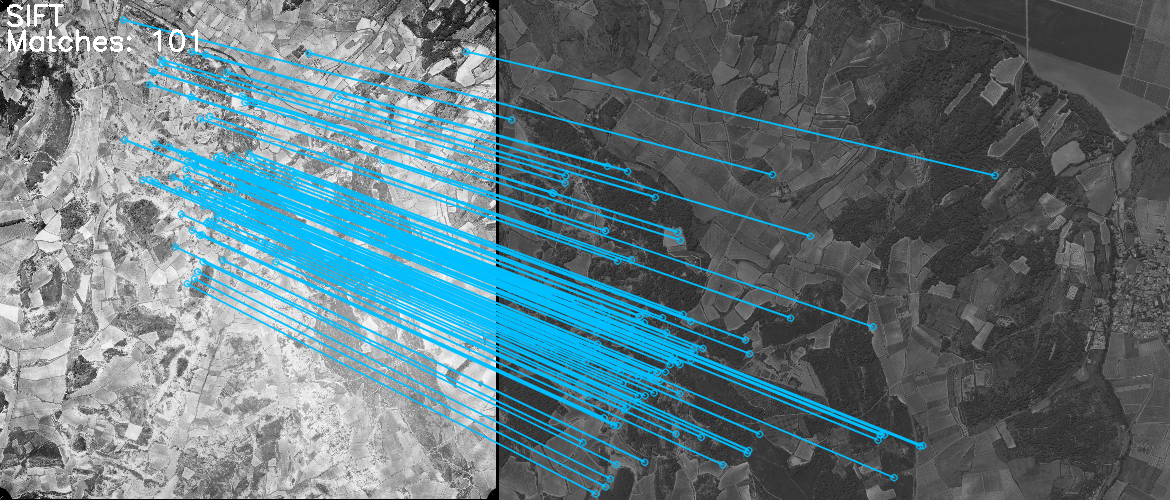
\includegraphics[width=6cm]{images/appendix/Homol-SIFT2Step_Test-Rough-2DRANSAC_OIS-Reech_IGNF_PVA_1-0__1971-06-21__C2844-0141_1971_FR2117_1124_15FD3425x00034_02911.png}
			\end{minipage}%
		}
		\subfigure[$SIFT_{orig}^{TotalMatches}$]{
			\begin{minipage}[t]{0.48\linewidth}
				\centering
				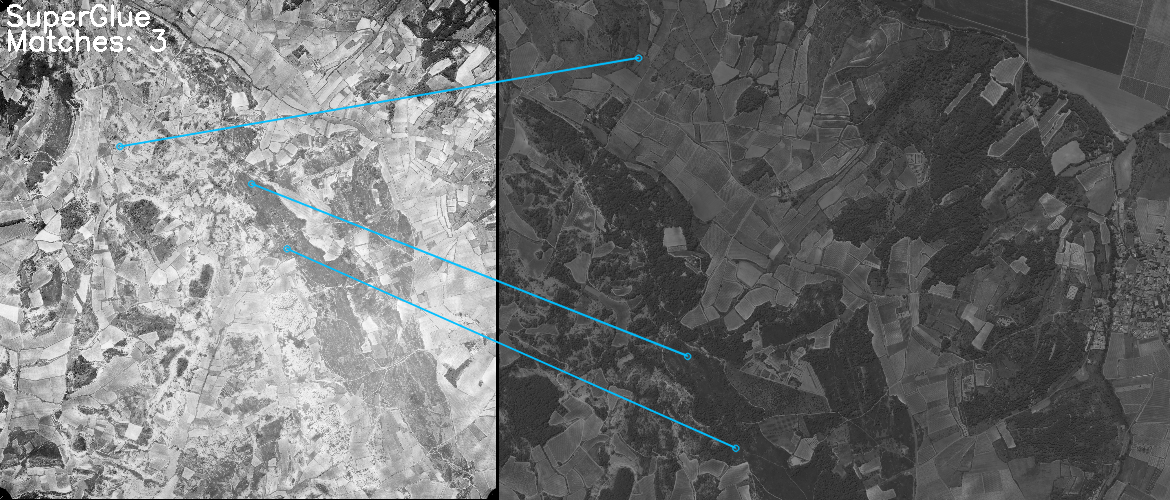
\includegraphics[width=6cm]{images/appendix/Homol-txt_OIS-Reech_IGNF_PVA_1-0__1971-06-21__C2844-0141_1971_FR2117_1124_15FD3425x00034_02911.png}
			\end{minipage}%
		}
		\caption{{\scriptsize Comparison between $SIFT_{ours}$ and $SIFT_{orig}$ on a pair of images from Pezenas 1971 and Pezenas 2015 individually. (a) Image pair to be matched, with red rectangles (\textcolor{red}{red rectangled to be drawn}) indicating the common zone. (b) Numbers of total matches, GT inliers and RANSAC inliers of $SIFT_{ours}$ and $SIFT_{orig}$. (c) Visualization of RANSAC inliers based on $SIFT_{ours}$. (d)Visualization of RANSAC inliers based on $SIFT_{orig}$.}}
		\label{Match result}
	\end{center}
\end{figure*} 

\section{Comparison on method $SIFT_{Ortho}$}
\begin{figure*}[htbp]
	\begin{center}
		\subfigure[Orthophotos]{
			\begin{minipage}[t]{0.48\linewidth}
				\centering
				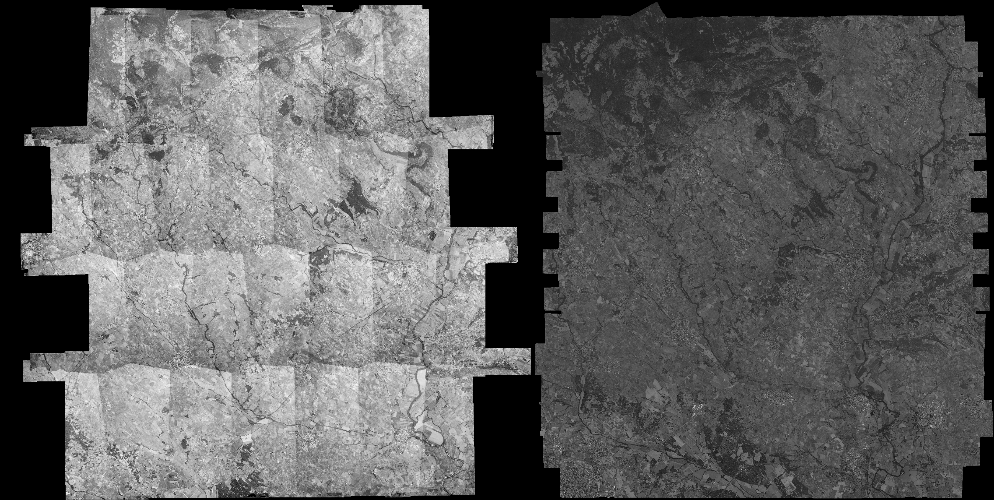
\includegraphics[width=7.5cm]{images/Chapitre3/Ortho-MEC-Malt_Tapas_1981_Ortho-MEC-Malt_2015.png}
			\end{minipage}%
		}
		\subfigure[Match number (\textit{Ortho})]{
			\begin{minipage}[t]{0.48\linewidth}
				\centering
				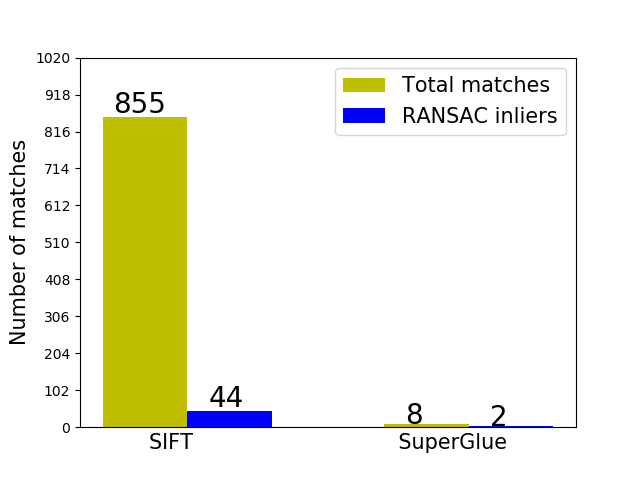
\includegraphics[width=4.8cm]{images/appendix/PlotCurves-SIFTComp_Ortho-MEC-Malt_Tapas_1981_Ortho-MEC-Malt_2015.png}
			\end{minipage}%
		}
		\subfigure[$SIFT_{ours}^{RANSAC Inliers}$]{
			\begin{minipage}[t]{0.48\linewidth}
				\centering
				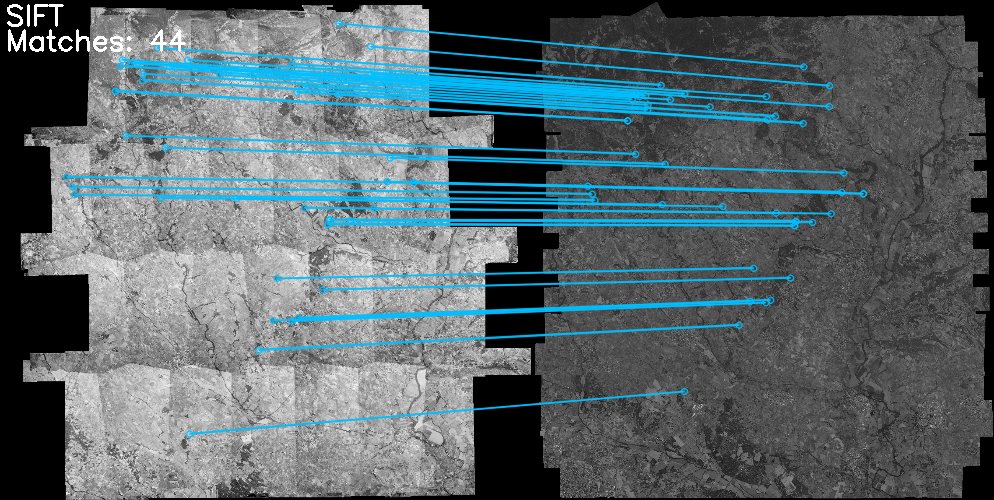
\includegraphics[width=6cm]{images/Chapitre3/Homol-SIFT2Step-Rough-2DRANSAC_Ortho-MEC-Malt_Tapas_1981_Ortho-MEC-Malt_2015.png}
			\end{minipage}%
		}
		\subfigure[$SIFT_{orig}^{TotalMatches}$]{
			\begin{minipage}[t]{0.48\linewidth}
				\centering
				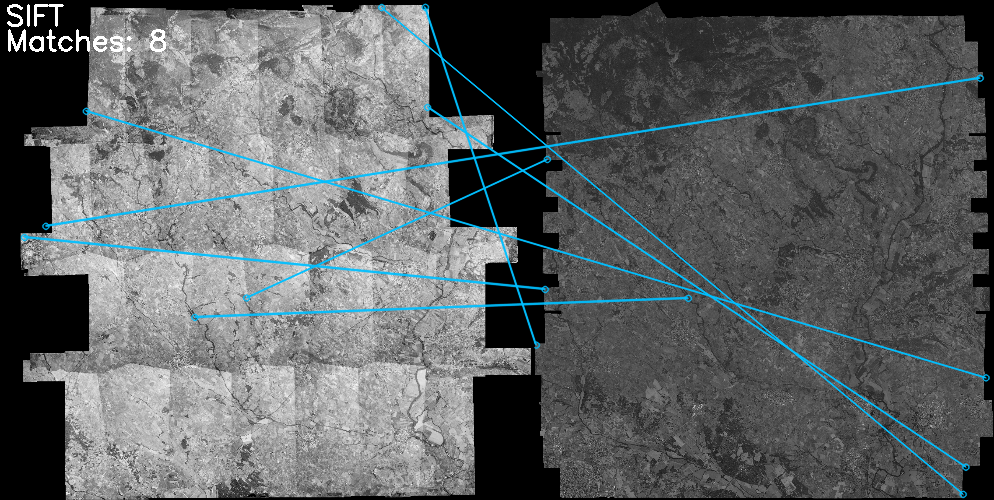
\includegraphics[width=6cm]{images/appendix/Homol-SIFT_Ortho-MEC-Malt_Tapas_1981_Ortho-MEC-Malt_2015.png}
			\end{minipage}%
		}
		\caption{Comparison between $SIFT_{ours}$ and $SIFT_{orig}$ on orthophotos from Pezenas 1981 and Pezenas 2015 individually. (a) Orthophotos to be matched, with red rectangles indicating the common zone. (b) Numbers of total matches, GT inliers and RANSAC inliers of $SIFT_{ours}$ and $SIFT_{orig}$. (c) Visualization of RANSAC inliers based on $SIFT_{ours}$. (d)Visualization of RANSAC inliers based on $SIFT_{orig}$.}
		\label{Match result}
	\end{center}
\end{figure*} 

\section{Comparison on method $SIFT_{DSM}$}
\begin{figure*}[htbp]
	\begin{center}
		\subfigure[DSMs]{
			\begin{minipage}[t]{0.65\linewidth}
				\centering
				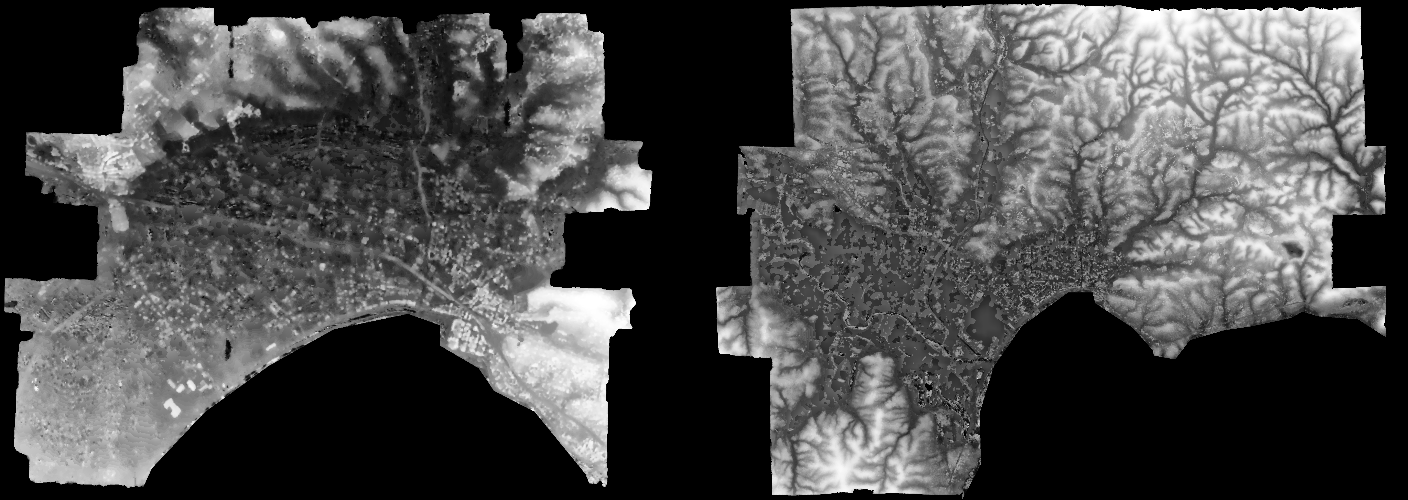
\includegraphics[width=8.8cm]{images/Chapitre3/MEC-Malt_Tapas_1954_MEC-Malt_2014.png}
			\end{minipage}%
		}
		\subfigure[Match number (\textit{DSM})]{
			\begin{minipage}[t]{0.3\linewidth}
				\centering
				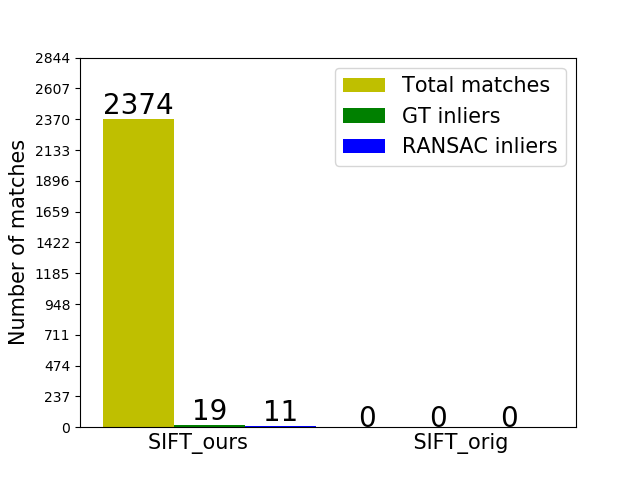
\includegraphics[width=4.8cm]{images/appendix/PlotCurves-SIFTComp_MEC-Malt_Tapas_1954_MEC-Malt_2014.png}
			\end{minipage}%
		}
		\subfigure[$SIFT_{ours}^{RANSAC Inliers}$]{
			\begin{minipage}[t]{0.48\linewidth}
				\centering
				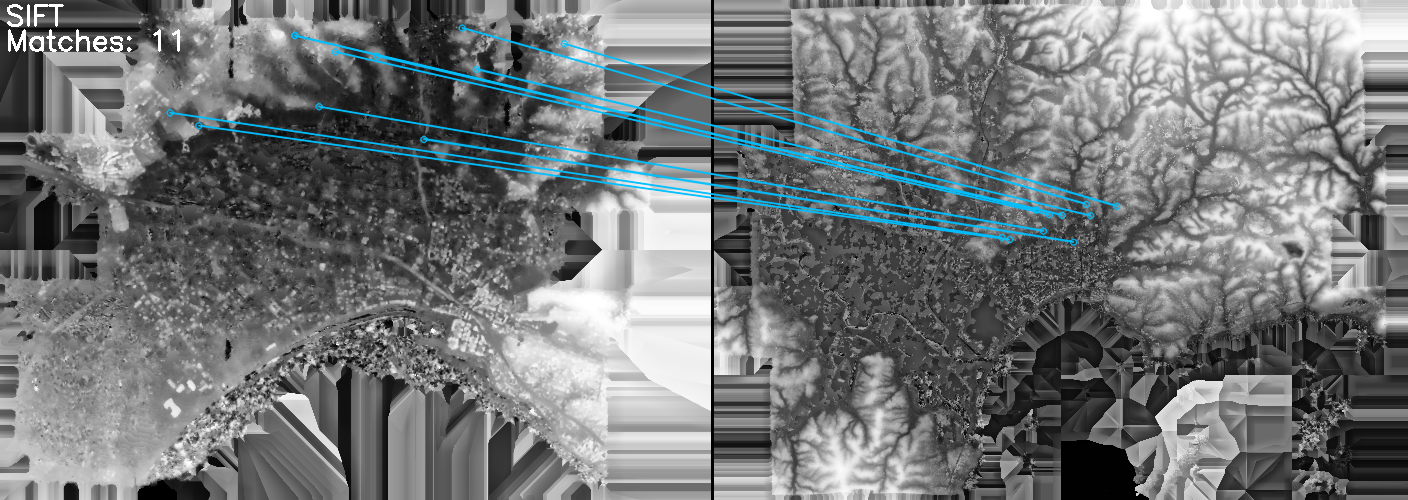
\includegraphics[width=6.8cm]{images/Chapitre3/Homol-SIFT2Step-Rough-2DRANSAC_MEC-Malt_Tapas_1954_MEC-Malt_2014.png}
			\end{minipage}%
		}
		\subfigure[$SIFT_{orig}^{TotalMatches}$]{
			\begin{minipage}[t]{0.48\linewidth}
				\centering
				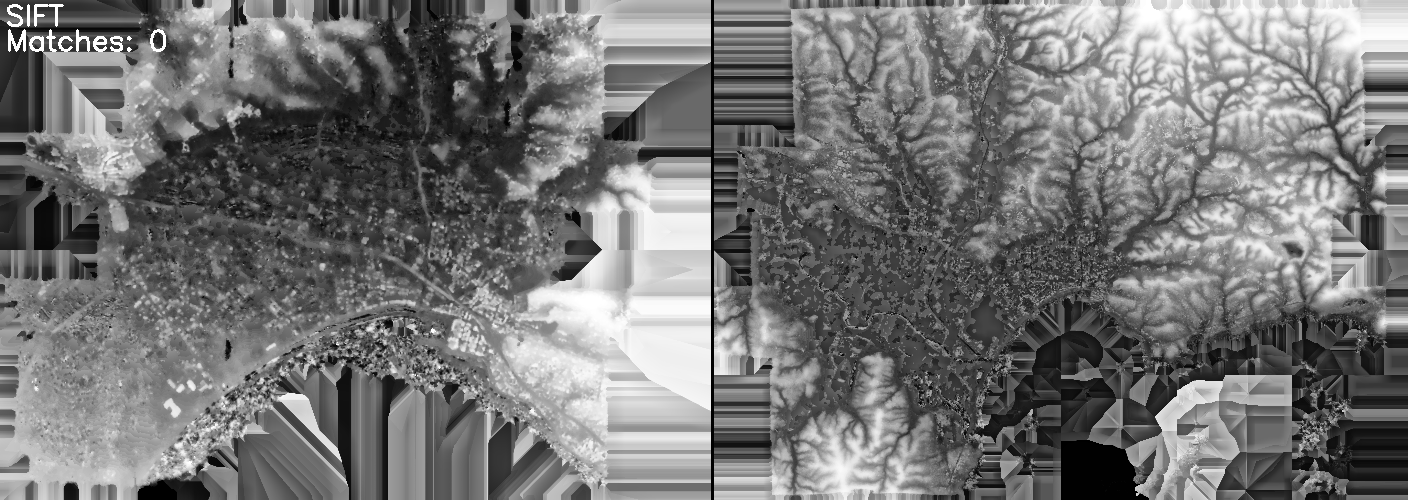
\includegraphics[width=6.8cm]{images/appendix/Homol-SIFT_MEC-Malt_Tapas_1954_MEC-Malt_2014.png}
			\end{minipage}%
		}
		\caption{Comparison between $SIFT_{ours}$ and $SIFT_{orig}$ on DSMs from Fr{\'e}jus 1954 and Fr{\'e}jus 2014 individually. (a) DSMs to be matched, with red rectangles indicating the common zone. (b) Numbers of total matches, GT inliers and RANSAC inliers of $SIFT_{ours}$ and $SIFT_{orig}$. (c) Visualization of RANSAC inliers based on $SIFT_{ours}$. (d)Visualization of RANSAC inliers based on $SIFT_{orig}$.}
		\label{Match result}
	\end{center}
\end{figure*} 


%And I cite myself to show by bibtex style file (two authors)~\cite{Commowick_MICCAI_2007}.
%This for other bibtex stye file : only one author~\cite{Oakes_RStat_1999} and many authors~\cite{Guimond_CVIU_2000}.